% Created by tikzDevice version 0.12.6 on 2024-02-25 14:51:27
% !TEX encoding = UTF-8 Unicode
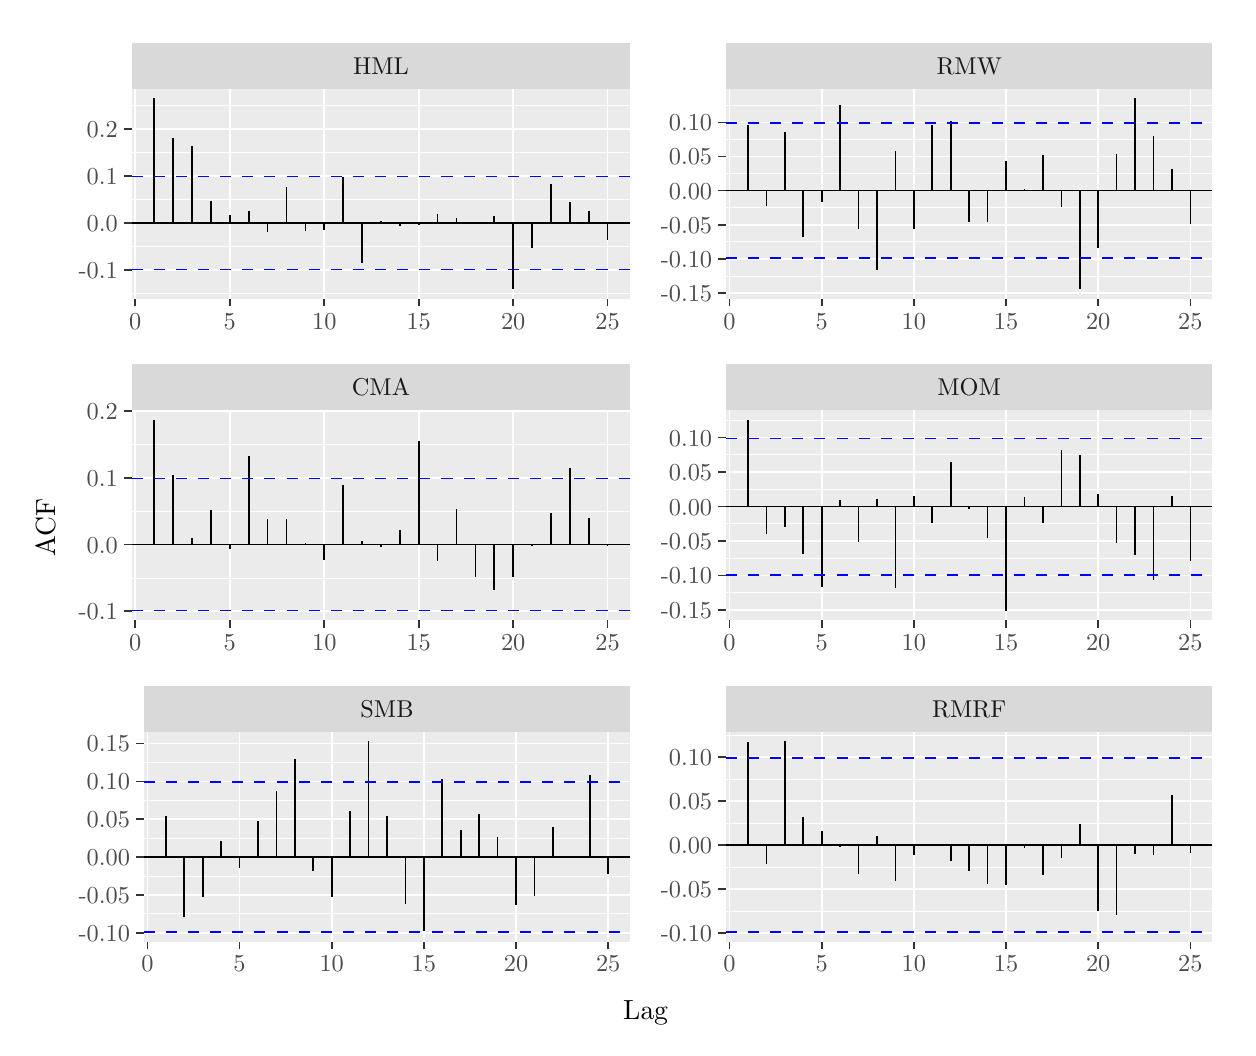
\begin{tikzpicture}[x=1pt,y=1pt]
\definecolor{fillColor}{RGB}{255,255,255}
\path[use as bounding box,fill=fillColor,fill opacity=0.00] (0,0) rectangle (433.62,361.35);
\begin{scope}
\path[clip] ( 12.91,245.20) rectangle (223.26,361.35);
\definecolor{drawColor}{RGB}{255,255,255}
\definecolor{fillColor}{RGB}{255,255,255}

\path[draw=drawColor,line width= 0.6pt,line join=round,line cap=round,fill=fillColor] ( 12.91,245.20) rectangle (223.26,361.35);
\end{scope}
\begin{scope}
\path[clip] ( 37.53,263.42) rectangle (217.76,339.28);
\definecolor{fillColor}{gray}{0.92}

\path[fill=fillColor] ( 37.53,263.42) rectangle (217.76,339.28);
\definecolor{drawColor}{RGB}{255,255,255}

\path[draw=drawColor,line width= 0.3pt,line join=round] ( 37.53,265.25) --
	(217.76,265.25);

\path[draw=drawColor,line width= 0.3pt,line join=round] ( 37.53,282.24) --
	(217.76,282.24);

\path[draw=drawColor,line width= 0.3pt,line join=round] ( 37.53,299.22) --
	(217.76,299.22);

\path[draw=drawColor,line width= 0.3pt,line join=round] ( 37.53,316.21) --
	(217.76,316.21);

\path[draw=drawColor,line width= 0.3pt,line join=round] ( 37.53,333.19) --
	(217.76,333.19);

\path[draw=drawColor,line width= 0.6pt,line join=round] ( 37.53,273.74) --
	(217.76,273.74);

\path[draw=drawColor,line width= 0.6pt,line join=round] ( 37.53,290.73) --
	(217.76,290.73);

\path[draw=drawColor,line width= 0.6pt,line join=round] ( 37.53,307.72) --
	(217.76,307.72);

\path[draw=drawColor,line width= 0.6pt,line join=round] ( 37.53,324.70) --
	(217.76,324.70);

\path[draw=drawColor,line width= 0.6pt,line join=round] ( 38.90,263.42) --
	( 38.90,339.28);

\path[draw=drawColor,line width= 0.6pt,line join=round] ( 73.03,263.42) --
	( 73.03,339.28);

\path[draw=drawColor,line width= 0.6pt,line join=round] (107.17,263.42) --
	(107.17,339.28);

\path[draw=drawColor,line width= 0.6pt,line join=round] (141.30,263.42) --
	(141.30,339.28);

\path[draw=drawColor,line width= 0.6pt,line join=round] (175.44,263.42) --
	(175.44,339.28);

\path[draw=drawColor,line width= 0.6pt,line join=round] (209.57,263.42) --
	(209.57,339.28);
\definecolor{drawColor}{RGB}{0,0,0}

\path[draw=drawColor,line width= 0.6pt,line join=round] ( 37.53,290.73) -- (217.76,290.73);

\path[draw=drawColor,line width= 0.6pt,line join=round] ( 45.73,290.73) -- ( 45.73,335.83);

\path[draw=drawColor,line width= 0.6pt,line join=round] ( 52.55,290.73) -- ( 52.55,321.43);

\path[draw=drawColor,line width= 0.6pt,line join=round] ( 59.38,290.73) -- ( 59.38,318.43);

\path[draw=drawColor,line width= 0.6pt,line join=round] ( 66.21,290.73) -- ( 66.21,298.76);

\path[draw=drawColor,line width= 0.6pt,line join=round] ( 73.03,290.73) -- ( 73.03,293.54);

\path[draw=drawColor,line width= 0.6pt,line join=round] ( 79.86,290.73) -- ( 79.86,294.99);

\path[draw=drawColor,line width= 0.6pt,line join=round] ( 86.69,290.73) -- ( 86.69,287.68);

\path[draw=drawColor,line width= 0.6pt,line join=round] ( 93.51,290.73) -- ( 93.51,303.92);

\path[draw=drawColor,line width= 0.6pt,line join=round] (100.34,290.73) -- (100.34,287.96);

\path[draw=drawColor,line width= 0.6pt,line join=round] (107.17,290.73) -- (107.17,288.35);

\path[draw=drawColor,line width= 0.6pt,line join=round] (114.00,290.73) -- (114.00,307.38);

\path[draw=drawColor,line width= 0.6pt,line join=round] (120.82,290.73) -- (120.82,276.36);

\path[draw=drawColor,line width= 0.6pt,line join=round] (127.65,290.73) -- (127.65,291.36);

\path[draw=drawColor,line width= 0.6pt,line join=round] (134.48,290.73) -- (134.48,289.50);

\path[draw=drawColor,line width= 0.6pt,line join=round] (141.30,290.73) -- (141.30,290.08);

\path[draw=drawColor,line width= 0.6pt,line join=round] (148.13,290.73) -- (148.13,293.90);

\path[draw=drawColor,line width= 0.6pt,line join=round] (154.96,290.73) -- (154.96,292.68);

\path[draw=drawColor,line width= 0.6pt,line join=round] (161.78,290.73) -- (161.78,290.30);

\path[draw=drawColor,line width= 0.6pt,line join=round] (168.61,290.73) -- (168.61,293.33);

\path[draw=drawColor,line width= 0.6pt,line join=round] (175.44,290.73) -- (175.44,266.87);

\path[draw=drawColor,line width= 0.6pt,line join=round] (182.26,290.73) -- (182.26,281.77);

\path[draw=drawColor,line width= 0.6pt,line join=round] (189.09,290.73) -- (189.09,304.71);

\path[draw=drawColor,line width= 0.6pt,line join=round] (195.92,290.73) -- (195.92,298.23);

\path[draw=drawColor,line width= 0.6pt,line join=round] (202.75,290.73) -- (202.75,294.98);

\path[draw=drawColor,line width= 0.6pt,line join=round] (209.57,290.73) -- (209.57,284.66);
\definecolor{drawColor}{RGB}{0,0,255}

\path[draw=drawColor,line width= 0.6pt,dash pattern=on 4pt off 4pt ,line join=round] ( 37.53,273.94) -- (217.76,273.94);

\path[draw=drawColor,line width= 0.6pt,dash pattern=on 4pt off 4pt ,line join=round] ( 37.53,307.52) -- (217.76,307.52);
\end{scope}
\begin{scope}
\path[clip] ( 37.53,339.28) rectangle (217.76,355.85);
\definecolor{fillColor}{gray}{0.85}

\path[fill=fillColor] ( 37.53,339.28) rectangle (217.76,355.85);
\definecolor{drawColor}{gray}{0.10}

\node[text=drawColor,anchor=base,inner sep=0pt, outer sep=0pt, scale=  0.88] at (127.65,344.53) {HML};
\end{scope}
\begin{scope}
\path[clip] (  0.00,  0.00) rectangle (433.62,361.35);
\definecolor{drawColor}{gray}{0.20}

\path[draw=drawColor,line width= 0.6pt,line join=round] ( 38.90,260.67) --
	( 38.90,263.42);

\path[draw=drawColor,line width= 0.6pt,line join=round] ( 73.03,260.67) --
	( 73.03,263.42);

\path[draw=drawColor,line width= 0.6pt,line join=round] (107.17,260.67) --
	(107.17,263.42);

\path[draw=drawColor,line width= 0.6pt,line join=round] (141.30,260.67) --
	(141.30,263.42);

\path[draw=drawColor,line width= 0.6pt,line join=round] (175.44,260.67) --
	(175.44,263.42);

\path[draw=drawColor,line width= 0.6pt,line join=round] (209.57,260.67) --
	(209.57,263.42);
\end{scope}
\begin{scope}
\path[clip] (  0.00,  0.00) rectangle (433.62,361.35);
\definecolor{drawColor}{gray}{0.30}

\node[text=drawColor,anchor=base,inner sep=0pt, outer sep=0pt, scale=  0.88] at ( 38.90,252.41) {0};

\node[text=drawColor,anchor=base,inner sep=0pt, outer sep=0pt, scale=  0.88] at ( 73.03,252.41) {5};

\node[text=drawColor,anchor=base,inner sep=0pt, outer sep=0pt, scale=  0.88] at (107.17,252.41) {10};

\node[text=drawColor,anchor=base,inner sep=0pt, outer sep=0pt, scale=  0.88] at (141.30,252.41) {15};

\node[text=drawColor,anchor=base,inner sep=0pt, outer sep=0pt, scale=  0.88] at (175.44,252.41) {20};

\node[text=drawColor,anchor=base,inner sep=0pt, outer sep=0pt, scale=  0.88] at (209.57,252.41) {25};
\end{scope}
\begin{scope}
\path[clip] (  0.00,  0.00) rectangle (433.62,361.35);
\definecolor{drawColor}{gray}{0.30}

\node[text=drawColor,anchor=base east,inner sep=0pt, outer sep=0pt, scale=  0.88] at ( 32.58,270.71) {-0.1};

\node[text=drawColor,anchor=base east,inner sep=0pt, outer sep=0pt, scale=  0.88] at ( 32.58,287.70) {0.0};

\node[text=drawColor,anchor=base east,inner sep=0pt, outer sep=0pt, scale=  0.88] at ( 32.58,304.69) {0.1};

\node[text=drawColor,anchor=base east,inner sep=0pt, outer sep=0pt, scale=  0.88] at ( 32.58,321.67) {0.2};
\end{scope}
\begin{scope}
\path[clip] (  0.00,  0.00) rectangle (433.62,361.35);
\definecolor{drawColor}{gray}{0.20}

\path[draw=drawColor,line width= 0.6pt,line join=round] ( 34.78,273.74) --
	( 37.53,273.74);

\path[draw=drawColor,line width= 0.6pt,line join=round] ( 34.78,290.73) --
	( 37.53,290.73);

\path[draw=drawColor,line width= 0.6pt,line join=round] ( 34.78,307.72) --
	( 37.53,307.72);

\path[draw=drawColor,line width= 0.6pt,line join=round] ( 34.78,324.70) --
	( 37.53,324.70);
\end{scope}
\begin{scope}
\path[clip] (223.26,245.20) rectangle (433.62,361.35);
\definecolor{drawColor}{RGB}{255,255,255}
\definecolor{fillColor}{RGB}{255,255,255}

\path[draw=drawColor,line width= 0.6pt,line join=round,line cap=round,fill=fillColor] (223.26,245.20) rectangle (433.62,361.35);
\end{scope}
\begin{scope}
\path[clip] (252.29,263.42) rectangle (428.12,339.28);
\definecolor{fillColor}{gray}{0.92}

\path[fill=fillColor] (252.29,263.42) rectangle (428.12,339.28);
\definecolor{drawColor}{RGB}{255,255,255}

\path[draw=drawColor,line width= 0.3pt,line join=round] (252.29,271.63) --
	(428.12,271.63);

\path[draw=drawColor,line width= 0.3pt,line join=round] (252.29,283.96) --
	(428.12,283.96);

\path[draw=drawColor,line width= 0.3pt,line join=round] (252.29,296.29) --
	(428.12,296.29);

\path[draw=drawColor,line width= 0.3pt,line join=round] (252.29,308.62) --
	(428.12,308.62);

\path[draw=drawColor,line width= 0.3pt,line join=round] (252.29,320.95) --
	(428.12,320.95);

\path[draw=drawColor,line width= 0.3pt,line join=round] (252.29,333.27) --
	(428.12,333.27);

\path[draw=drawColor,line width= 0.6pt,line join=round] (252.29,265.46) --
	(428.12,265.46);

\path[draw=drawColor,line width= 0.6pt,line join=round] (252.29,277.79) --
	(428.12,277.79);

\path[draw=drawColor,line width= 0.6pt,line join=round] (252.29,290.12) --
	(428.12,290.12);

\path[draw=drawColor,line width= 0.6pt,line join=round] (252.29,302.45) --
	(428.12,302.45);

\path[draw=drawColor,line width= 0.6pt,line join=round] (252.29,314.78) --
	(428.12,314.78);

\path[draw=drawColor,line width= 0.6pt,line join=round] (252.29,327.11) --
	(428.12,327.11);

\path[draw=drawColor,line width= 0.6pt,line join=round] (253.62,263.42) --
	(253.62,339.28);

\path[draw=drawColor,line width= 0.6pt,line join=round] (286.92,263.42) --
	(286.92,339.28);

\path[draw=drawColor,line width= 0.6pt,line join=round] (320.22,263.42) --
	(320.22,339.28);

\path[draw=drawColor,line width= 0.6pt,line join=round] (353.52,263.42) --
	(353.52,339.28);

\path[draw=drawColor,line width= 0.6pt,line join=round] (386.83,263.42) --
	(386.83,339.28);

\path[draw=drawColor,line width= 0.6pt,line join=round] (420.13,263.42) --
	(420.13,339.28);
\definecolor{drawColor}{RGB}{0,0,0}

\path[draw=drawColor,line width= 0.6pt,line join=round] (252.29,302.45) -- (428.12,302.45);

\path[draw=drawColor,line width= 0.6pt,line join=round] (260.28,302.45) -- (260.28,326.14);

\path[draw=drawColor,line width= 0.6pt,line join=round] (266.94,302.45) -- (266.94,297.04);

\path[draw=drawColor,line width= 0.6pt,line join=round] (273.60,302.45) -- (273.60,323.62);

\path[draw=drawColor,line width= 0.6pt,line join=round] (280.26,302.45) -- (280.26,285.77);

\path[draw=drawColor,line width= 0.6pt,line join=round] (286.92,302.45) -- (286.92,298.49);

\path[draw=drawColor,line width= 0.6pt,line join=round] (293.58,302.45) -- (293.58,333.58);

\path[draw=drawColor,line width= 0.6pt,line join=round] (300.24,302.45) -- (300.24,288.71);

\path[draw=drawColor,line width= 0.6pt,line join=round] (306.90,302.45) -- (306.90,273.85);

\path[draw=drawColor,line width= 0.6pt,line join=round] (313.56,302.45) -- (313.56,316.96);

\path[draw=drawColor,line width= 0.6pt,line join=round] (320.22,302.45) -- (320.22,288.61);

\path[draw=drawColor,line width= 0.6pt,line join=round] (326.88,302.45) -- (326.88,326.12);

\path[draw=drawColor,line width= 0.6pt,line join=round] (333.54,302.45) -- (333.54,327.62);

\path[draw=drawColor,line width= 0.6pt,line join=round] (340.20,302.45) -- (340.20,291.09);

\path[draw=drawColor,line width= 0.6pt,line join=round] (346.86,302.45) -- (346.86,290.95);

\path[draw=drawColor,line width= 0.6pt,line join=round] (353.52,302.45) -- (353.52,313.17);

\path[draw=drawColor,line width= 0.6pt,line join=round] (360.18,302.45) -- (360.18,303.11);

\path[draw=drawColor,line width= 0.6pt,line join=round] (366.85,302.45) -- (366.85,315.38);

\path[draw=drawColor,line width= 0.6pt,line join=round] (373.51,302.45) -- (373.51,296.45);

\path[draw=drawColor,line width= 0.6pt,line join=round] (380.17,302.45) -- (380.17,266.87);

\path[draw=drawColor,line width= 0.6pt,line join=round] (386.83,302.45) -- (386.83,281.57);

\path[draw=drawColor,line width= 0.6pt,line join=round] (393.49,302.45) -- (393.49,315.55);

\path[draw=drawColor,line width= 0.6pt,line join=round] (400.15,302.45) -- (400.15,335.83);

\path[draw=drawColor,line width= 0.6pt,line join=round] (406.81,302.45) -- (406.81,322.22);

\path[draw=drawColor,line width= 0.6pt,line join=round] (413.47,302.45) -- (413.47,310.33);

\path[draw=drawColor,line width= 0.6pt,line join=round] (420.13,302.45) -- (420.13,290.32);
\definecolor{drawColor}{RGB}{0,0,255}

\path[draw=drawColor,line width= 0.6pt,dash pattern=on 4pt off 4pt ,line join=round] (252.29,278.07) -- (428.12,278.07);

\path[draw=drawColor,line width= 0.6pt,dash pattern=on 4pt off 4pt ,line join=round] (252.29,326.83) -- (428.12,326.83);
\end{scope}
\begin{scope}
\path[clip] (252.29,339.28) rectangle (428.12,355.85);
\definecolor{fillColor}{gray}{0.85}

\path[fill=fillColor] (252.29,339.28) rectangle (428.12,355.85);
\definecolor{drawColor}{gray}{0.10}

\node[text=drawColor,anchor=base,inner sep=0pt, outer sep=0pt, scale=  0.88] at (340.20,344.53) {RMW};
\end{scope}
\begin{scope}
\path[clip] (  0.00,  0.00) rectangle (433.62,361.35);
\definecolor{drawColor}{gray}{0.20}

\path[draw=drawColor,line width= 0.6pt,line join=round] (253.62,260.67) --
	(253.62,263.42);

\path[draw=drawColor,line width= 0.6pt,line join=round] (286.92,260.67) --
	(286.92,263.42);

\path[draw=drawColor,line width= 0.6pt,line join=round] (320.22,260.67) --
	(320.22,263.42);

\path[draw=drawColor,line width= 0.6pt,line join=round] (353.52,260.67) --
	(353.52,263.42);

\path[draw=drawColor,line width= 0.6pt,line join=round] (386.83,260.67) --
	(386.83,263.42);

\path[draw=drawColor,line width= 0.6pt,line join=round] (420.13,260.67) --
	(420.13,263.42);
\end{scope}
\begin{scope}
\path[clip] (  0.00,  0.00) rectangle (433.62,361.35);
\definecolor{drawColor}{gray}{0.30}

\node[text=drawColor,anchor=base,inner sep=0pt, outer sep=0pt, scale=  0.88] at (253.62,252.41) {0};

\node[text=drawColor,anchor=base,inner sep=0pt, outer sep=0pt, scale=  0.88] at (286.92,252.41) {5};

\node[text=drawColor,anchor=base,inner sep=0pt, outer sep=0pt, scale=  0.88] at (320.22,252.41) {10};

\node[text=drawColor,anchor=base,inner sep=0pt, outer sep=0pt, scale=  0.88] at (353.52,252.41) {15};

\node[text=drawColor,anchor=base,inner sep=0pt, outer sep=0pt, scale=  0.88] at (386.83,252.41) {20};

\node[text=drawColor,anchor=base,inner sep=0pt, outer sep=0pt, scale=  0.88] at (420.13,252.41) {25};
\end{scope}
\begin{scope}
\path[clip] (  0.00,  0.00) rectangle (433.62,361.35);
\definecolor{drawColor}{gray}{0.30}

\node[text=drawColor,anchor=base east,inner sep=0pt, outer sep=0pt, scale=  0.88] at (247.34,262.43) {-0.15};

\node[text=drawColor,anchor=base east,inner sep=0pt, outer sep=0pt, scale=  0.88] at (247.34,274.76) {-0.10};

\node[text=drawColor,anchor=base east,inner sep=0pt, outer sep=0pt, scale=  0.88] at (247.34,287.09) {-0.05};

\node[text=drawColor,anchor=base east,inner sep=0pt, outer sep=0pt, scale=  0.88] at (247.34,299.42) {0.00};

\node[text=drawColor,anchor=base east,inner sep=0pt, outer sep=0pt, scale=  0.88] at (247.34,311.75) {0.05};

\node[text=drawColor,anchor=base east,inner sep=0pt, outer sep=0pt, scale=  0.88] at (247.34,324.08) {0.10};
\end{scope}
\begin{scope}
\path[clip] (  0.00,  0.00) rectangle (433.62,361.35);
\definecolor{drawColor}{gray}{0.20}

\path[draw=drawColor,line width= 0.6pt,line join=round] (249.54,265.46) --
	(252.29,265.46);

\path[draw=drawColor,line width= 0.6pt,line join=round] (249.54,277.79) --
	(252.29,277.79);

\path[draw=drawColor,line width= 0.6pt,line join=round] (249.54,290.12) --
	(252.29,290.12);

\path[draw=drawColor,line width= 0.6pt,line join=round] (249.54,302.45) --
	(252.29,302.45);

\path[draw=drawColor,line width= 0.6pt,line join=round] (249.54,314.78) --
	(252.29,314.78);

\path[draw=drawColor,line width= 0.6pt,line join=round] (249.54,327.11) --
	(252.29,327.11);
\end{scope}
\begin{scope}
\path[clip] ( 12.91,129.06) rectangle (223.26,245.20);
\definecolor{drawColor}{RGB}{255,255,255}
\definecolor{fillColor}{RGB}{255,255,255}

\path[draw=drawColor,line width= 0.6pt,line join=round,line cap=round,fill=fillColor] ( 12.91,129.06) rectangle (223.26,245.20);
\end{scope}
\begin{scope}
\path[clip] ( 37.53,147.28) rectangle (217.76,223.13);
\definecolor{fillColor}{gray}{0.92}

\path[fill=fillColor] ( 37.53,147.28) rectangle (217.76,223.13);
\definecolor{drawColor}{RGB}{255,255,255}

\path[draw=drawColor,line width= 0.3pt,line join=round] ( 37.53,162.50) --
	(217.76,162.50);

\path[draw=drawColor,line width= 0.3pt,line join=round] ( 37.53,186.61) --
	(217.76,186.61);

\path[draw=drawColor,line width= 0.3pt,line join=round] ( 37.53,210.71) --
	(217.76,210.71);

\path[draw=drawColor,line width= 0.6pt,line join=round] ( 37.53,150.45) --
	(217.76,150.45);

\path[draw=drawColor,line width= 0.6pt,line join=round] ( 37.53,174.55) --
	(217.76,174.55);

\path[draw=drawColor,line width= 0.6pt,line join=round] ( 37.53,198.66) --
	(217.76,198.66);

\path[draw=drawColor,line width= 0.6pt,line join=round] ( 37.53,222.76) --
	(217.76,222.76);

\path[draw=drawColor,line width= 0.6pt,line join=round] ( 38.90,147.28) --
	( 38.90,223.13);

\path[draw=drawColor,line width= 0.6pt,line join=round] ( 73.03,147.28) --
	( 73.03,223.13);

\path[draw=drawColor,line width= 0.6pt,line join=round] (107.17,147.28) --
	(107.17,223.13);

\path[draw=drawColor,line width= 0.6pt,line join=round] (141.30,147.28) --
	(141.30,223.13);

\path[draw=drawColor,line width= 0.6pt,line join=round] (175.44,147.28) --
	(175.44,223.13);

\path[draw=drawColor,line width= 0.6pt,line join=round] (209.57,147.28) --
	(209.57,223.13);
\definecolor{drawColor}{RGB}{0,0,0}

\path[draw=drawColor,line width= 0.6pt,line join=round] ( 37.53,174.55) -- (217.76,174.55);

\path[draw=drawColor,line width= 0.6pt,line join=round] ( 45.73,174.55) -- ( 45.73,219.68);

\path[draw=drawColor,line width= 0.6pt,line join=round] ( 52.55,174.55) -- ( 52.55,199.74);

\path[draw=drawColor,line width= 0.6pt,line join=round] ( 59.38,174.55) -- ( 59.38,177.11);

\path[draw=drawColor,line width= 0.6pt,line join=round] ( 66.21,174.55) -- ( 66.21,187.23);

\path[draw=drawColor,line width= 0.6pt,line join=round] ( 73.03,174.55) -- ( 73.03,172.99);

\path[draw=drawColor,line width= 0.6pt,line join=round] ( 79.86,174.55) -- ( 79.86,206.57);

\path[draw=drawColor,line width= 0.6pt,line join=round] ( 86.69,174.55) -- ( 86.69,183.69);

\path[draw=drawColor,line width= 0.6pt,line join=round] ( 93.51,174.55) -- ( 93.51,183.65);

\path[draw=drawColor,line width= 0.6pt,line join=round] (100.34,174.55) -- (100.34,175.11);

\path[draw=drawColor,line width= 0.6pt,line join=round] (107.17,174.55) -- (107.17,169.04);

\path[draw=drawColor,line width= 0.6pt,line join=round] (114.00,174.55) -- (114.00,196.19);

\path[draw=drawColor,line width= 0.6pt,line join=round] (120.82,174.55) -- (120.82,175.89);

\path[draw=drawColor,line width= 0.6pt,line join=round] (127.65,174.55) -- (127.65,173.64);

\path[draw=drawColor,line width= 0.6pt,line join=round] (134.48,174.55) -- (134.48,180.00);

\path[draw=drawColor,line width= 0.6pt,line join=round] (141.30,174.55) -- (141.30,211.82);

\path[draw=drawColor,line width= 0.6pt,line join=round] (148.13,174.55) -- (148.13,168.51);

\path[draw=drawColor,line width= 0.6pt,line join=round] (154.96,174.55) -- (154.96,187.37);

\path[draw=drawColor,line width= 0.6pt,line join=round] (161.78,174.55) -- (161.78,162.72);

\path[draw=drawColor,line width= 0.6pt,line join=round] (168.61,174.55) -- (168.61,158.07);

\path[draw=drawColor,line width= 0.6pt,line join=round] (175.44,174.55) -- (175.44,162.86);

\path[draw=drawColor,line width= 0.6pt,line join=round] (182.26,174.55) -- (182.26,174.26);

\path[draw=drawColor,line width= 0.6pt,line join=round] (189.09,174.55) -- (189.09,185.90);

\path[draw=drawColor,line width= 0.6pt,line join=round] (195.92,174.55) -- (195.92,202.35);

\path[draw=drawColor,line width= 0.6pt,line join=round] (202.75,174.55) -- (202.75,184.04);

\path[draw=drawColor,line width= 0.6pt,line join=round] (209.57,174.55) -- (209.57,174.16);
\definecolor{drawColor}{RGB}{0,0,255}

\path[draw=drawColor,line width= 0.6pt,dash pattern=on 4pt off 4pt ,line join=round] ( 37.53,150.73) -- (217.76,150.73);

\path[draw=drawColor,line width= 0.6pt,dash pattern=on 4pt off 4pt ,line join=round] ( 37.53,198.38) -- (217.76,198.38);
\end{scope}
\begin{scope}
\path[clip] ( 37.53,223.13) rectangle (217.76,239.70);
\definecolor{fillColor}{gray}{0.85}

\path[fill=fillColor] ( 37.53,223.13) rectangle (217.76,239.70);
\definecolor{drawColor}{gray}{0.10}

\node[text=drawColor,anchor=base,inner sep=0pt, outer sep=0pt, scale=  0.88] at (127.65,228.39) {CMA};
\end{scope}
\begin{scope}
\path[clip] (  0.00,  0.00) rectangle (433.62,361.35);
\definecolor{drawColor}{gray}{0.20}

\path[draw=drawColor,line width= 0.6pt,line join=round] ( 38.90,144.53) --
	( 38.90,147.28);

\path[draw=drawColor,line width= 0.6pt,line join=round] ( 73.03,144.53) --
	( 73.03,147.28);

\path[draw=drawColor,line width= 0.6pt,line join=round] (107.17,144.53) --
	(107.17,147.28);

\path[draw=drawColor,line width= 0.6pt,line join=round] (141.30,144.53) --
	(141.30,147.28);

\path[draw=drawColor,line width= 0.6pt,line join=round] (175.44,144.53) --
	(175.44,147.28);

\path[draw=drawColor,line width= 0.6pt,line join=round] (209.57,144.53) --
	(209.57,147.28);
\end{scope}
\begin{scope}
\path[clip] (  0.00,  0.00) rectangle (433.62,361.35);
\definecolor{drawColor}{gray}{0.30}

\node[text=drawColor,anchor=base,inner sep=0pt, outer sep=0pt, scale=  0.88] at ( 38.90,136.27) {0};

\node[text=drawColor,anchor=base,inner sep=0pt, outer sep=0pt, scale=  0.88] at ( 73.03,136.27) {5};

\node[text=drawColor,anchor=base,inner sep=0pt, outer sep=0pt, scale=  0.88] at (107.17,136.27) {10};

\node[text=drawColor,anchor=base,inner sep=0pt, outer sep=0pt, scale=  0.88] at (141.30,136.27) {15};

\node[text=drawColor,anchor=base,inner sep=0pt, outer sep=0pt, scale=  0.88] at (175.44,136.27) {20};

\node[text=drawColor,anchor=base,inner sep=0pt, outer sep=0pt, scale=  0.88] at (209.57,136.27) {25};
\end{scope}
\begin{scope}
\path[clip] (  0.00,  0.00) rectangle (433.62,361.35);
\definecolor{drawColor}{gray}{0.30}

\node[text=drawColor,anchor=base east,inner sep=0pt, outer sep=0pt, scale=  0.88] at ( 32.58,147.42) {-0.1};

\node[text=drawColor,anchor=base east,inner sep=0pt, outer sep=0pt, scale=  0.88] at ( 32.58,171.52) {0.0};

\node[text=drawColor,anchor=base east,inner sep=0pt, outer sep=0pt, scale=  0.88] at ( 32.58,195.63) {0.1};

\node[text=drawColor,anchor=base east,inner sep=0pt, outer sep=0pt, scale=  0.88] at ( 32.58,219.73) {0.2};
\end{scope}
\begin{scope}
\path[clip] (  0.00,  0.00) rectangle (433.62,361.35);
\definecolor{drawColor}{gray}{0.20}

\path[draw=drawColor,line width= 0.6pt,line join=round] ( 34.78,150.45) --
	( 37.53,150.45);

\path[draw=drawColor,line width= 0.6pt,line join=round] ( 34.78,174.55) --
	( 37.53,174.55);

\path[draw=drawColor,line width= 0.6pt,line join=round] ( 34.78,198.66) --
	( 37.53,198.66);

\path[draw=drawColor,line width= 0.6pt,line join=round] ( 34.78,222.76) --
	( 37.53,222.76);
\end{scope}
\begin{scope}
\path[clip] (223.26,129.06) rectangle (433.62,245.20);
\definecolor{drawColor}{RGB}{255,255,255}
\definecolor{fillColor}{RGB}{255,255,255}

\path[draw=drawColor,line width= 0.6pt,line join=round,line cap=round,fill=fillColor] (223.26,129.06) rectangle (433.62,245.20);
\end{scope}
\begin{scope}
\path[clip] (252.29,147.28) rectangle (428.12,223.13);
\definecolor{fillColor}{gray}{0.92}

\path[fill=fillColor] (252.29,147.28) rectangle (428.12,223.13);
\definecolor{drawColor}{RGB}{255,255,255}

\path[draw=drawColor,line width= 0.3pt,line join=round] (252.29,157.13) --
	(428.12,157.13);

\path[draw=drawColor,line width= 0.3pt,line join=round] (252.29,169.59) --
	(428.12,169.59);

\path[draw=drawColor,line width= 0.3pt,line join=round] (252.29,182.05) --
	(428.12,182.05);

\path[draw=drawColor,line width= 0.3pt,line join=round] (252.29,194.51) --
	(428.12,194.51);

\path[draw=drawColor,line width= 0.3pt,line join=round] (252.29,206.97) --
	(428.12,206.97);

\path[draw=drawColor,line width= 0.3pt,line join=round] (252.29,219.44) --
	(428.12,219.44);

\path[draw=drawColor,line width= 0.6pt,line join=round] (252.29,150.90) --
	(428.12,150.90);

\path[draw=drawColor,line width= 0.6pt,line join=round] (252.29,163.36) --
	(428.12,163.36);

\path[draw=drawColor,line width= 0.6pt,line join=round] (252.29,175.82) --
	(428.12,175.82);

\path[draw=drawColor,line width= 0.6pt,line join=round] (252.29,188.28) --
	(428.12,188.28);

\path[draw=drawColor,line width= 0.6pt,line join=round] (252.29,200.74) --
	(428.12,200.74);

\path[draw=drawColor,line width= 0.6pt,line join=round] (252.29,213.20) --
	(428.12,213.20);

\path[draw=drawColor,line width= 0.6pt,line join=round] (253.62,147.28) --
	(253.62,223.13);

\path[draw=drawColor,line width= 0.6pt,line join=round] (286.92,147.28) --
	(286.92,223.13);

\path[draw=drawColor,line width= 0.6pt,line join=round] (320.22,147.28) --
	(320.22,223.13);

\path[draw=drawColor,line width= 0.6pt,line join=round] (353.52,147.28) --
	(353.52,223.13);

\path[draw=drawColor,line width= 0.6pt,line join=round] (386.83,147.28) --
	(386.83,223.13);

\path[draw=drawColor,line width= 0.6pt,line join=round] (420.13,147.28) --
	(420.13,223.13);
\definecolor{drawColor}{RGB}{0,0,0}

\path[draw=drawColor,line width= 0.6pt,line join=round] (252.29,188.28) -- (428.12,188.28);

\path[draw=drawColor,line width= 0.6pt,line join=round] (260.28,188.28) -- (260.28,219.68);

\path[draw=drawColor,line width= 0.6pt,line join=round] (266.94,188.28) -- (266.94,178.54);

\path[draw=drawColor,line width= 0.6pt,line join=round] (273.60,188.28) -- (273.60,180.92);

\path[draw=drawColor,line width= 0.6pt,line join=round] (280.26,188.28) -- (280.26,171.00);

\path[draw=drawColor,line width= 0.6pt,line join=round] (286.92,188.28) -- (286.92,159.13);

\path[draw=drawColor,line width= 0.6pt,line join=round] (293.58,188.28) -- (293.58,190.62);

\path[draw=drawColor,line width= 0.6pt,line join=round] (300.24,188.28) -- (300.24,175.67);

\path[draw=drawColor,line width= 0.6pt,line join=round] (306.90,188.28) -- (306.90,191.03);

\path[draw=drawColor,line width= 0.6pt,line join=round] (313.56,188.28) -- (313.56,158.99);

\path[draw=drawColor,line width= 0.6pt,line join=round] (320.22,188.28) -- (320.22,192.18);

\path[draw=drawColor,line width= 0.6pt,line join=round] (326.88,188.28) -- (326.88,182.37);

\path[draw=drawColor,line width= 0.6pt,line join=round] (333.54,188.28) -- (333.54,204.54);

\path[draw=drawColor,line width= 0.6pt,line join=round] (340.20,188.28) -- (340.20,187.60);

\path[draw=drawColor,line width= 0.6pt,line join=round] (346.86,188.28) -- (346.86,176.89);

\path[draw=drawColor,line width= 0.6pt,line join=round] (353.52,188.28) -- (353.52,150.73);

\path[draw=drawColor,line width= 0.6pt,line join=round] (360.18,188.28) -- (360.18,191.85);

\path[draw=drawColor,line width= 0.6pt,line join=round] (366.85,188.28) -- (366.85,182.21);

\path[draw=drawColor,line width= 0.6pt,line join=round] (373.51,188.28) -- (373.51,208.71);

\path[draw=drawColor,line width= 0.6pt,line join=round] (380.17,188.28) -- (380.17,206.92);

\path[draw=drawColor,line width= 0.6pt,line join=round] (386.83,188.28) -- (386.83,193.01);

\path[draw=drawColor,line width= 0.6pt,line join=round] (393.49,188.28) -- (393.49,175.08);

\path[draw=drawColor,line width= 0.6pt,line join=round] (400.15,188.28) -- (400.15,170.64);

\path[draw=drawColor,line width= 0.6pt,line join=round] (406.81,188.28) -- (406.81,161.77);

\path[draw=drawColor,line width= 0.6pt,line join=round] (413.47,188.28) -- (413.47,192.00);

\path[draw=drawColor,line width= 0.6pt,line join=round] (420.13,188.28) -- (420.13,168.81);
\definecolor{drawColor}{RGB}{0,0,255}

\path[draw=drawColor,line width= 0.6pt,dash pattern=on 4pt off 4pt ,line join=round] (252.29,163.64) -- (428.12,163.64);

\path[draw=drawColor,line width= 0.6pt,dash pattern=on 4pt off 4pt ,line join=round] (252.29,212.92) -- (428.12,212.92);
\end{scope}
\begin{scope}
\path[clip] (252.29,223.13) rectangle (428.12,239.70);
\definecolor{fillColor}{gray}{0.85}

\path[fill=fillColor] (252.29,223.13) rectangle (428.12,239.70);
\definecolor{drawColor}{gray}{0.10}

\node[text=drawColor,anchor=base,inner sep=0pt, outer sep=0pt, scale=  0.88] at (340.20,228.39) {MOM};
\end{scope}
\begin{scope}
\path[clip] (  0.00,  0.00) rectangle (433.62,361.35);
\definecolor{drawColor}{gray}{0.20}

\path[draw=drawColor,line width= 0.6pt,line join=round] (253.62,144.53) --
	(253.62,147.28);

\path[draw=drawColor,line width= 0.6pt,line join=round] (286.92,144.53) --
	(286.92,147.28);

\path[draw=drawColor,line width= 0.6pt,line join=round] (320.22,144.53) --
	(320.22,147.28);

\path[draw=drawColor,line width= 0.6pt,line join=round] (353.52,144.53) --
	(353.52,147.28);

\path[draw=drawColor,line width= 0.6pt,line join=round] (386.83,144.53) --
	(386.83,147.28);

\path[draw=drawColor,line width= 0.6pt,line join=round] (420.13,144.53) --
	(420.13,147.28);
\end{scope}
\begin{scope}
\path[clip] (  0.00,  0.00) rectangle (433.62,361.35);
\definecolor{drawColor}{gray}{0.30}

\node[text=drawColor,anchor=base,inner sep=0pt, outer sep=0pt, scale=  0.88] at (253.62,136.27) {0};

\node[text=drawColor,anchor=base,inner sep=0pt, outer sep=0pt, scale=  0.88] at (286.92,136.27) {5};

\node[text=drawColor,anchor=base,inner sep=0pt, outer sep=0pt, scale=  0.88] at (320.22,136.27) {10};

\node[text=drawColor,anchor=base,inner sep=0pt, outer sep=0pt, scale=  0.88] at (353.52,136.27) {15};

\node[text=drawColor,anchor=base,inner sep=0pt, outer sep=0pt, scale=  0.88] at (386.83,136.27) {20};

\node[text=drawColor,anchor=base,inner sep=0pt, outer sep=0pt, scale=  0.88] at (420.13,136.27) {25};
\end{scope}
\begin{scope}
\path[clip] (  0.00,  0.00) rectangle (433.62,361.35);
\definecolor{drawColor}{gray}{0.30}

\node[text=drawColor,anchor=base east,inner sep=0pt, outer sep=0pt, scale=  0.88] at (247.34,147.86) {-0.15};

\node[text=drawColor,anchor=base east,inner sep=0pt, outer sep=0pt, scale=  0.88] at (247.34,160.33) {-0.10};

\node[text=drawColor,anchor=base east,inner sep=0pt, outer sep=0pt, scale=  0.88] at (247.34,172.79) {-0.05};

\node[text=drawColor,anchor=base east,inner sep=0pt, outer sep=0pt, scale=  0.88] at (247.34,185.25) {0.00};

\node[text=drawColor,anchor=base east,inner sep=0pt, outer sep=0pt, scale=  0.88] at (247.34,197.71) {0.05};

\node[text=drawColor,anchor=base east,inner sep=0pt, outer sep=0pt, scale=  0.88] at (247.34,210.17) {0.10};
\end{scope}
\begin{scope}
\path[clip] (  0.00,  0.00) rectangle (433.62,361.35);
\definecolor{drawColor}{gray}{0.20}

\path[draw=drawColor,line width= 0.6pt,line join=round] (249.54,150.90) --
	(252.29,150.90);

\path[draw=drawColor,line width= 0.6pt,line join=round] (249.54,163.36) --
	(252.29,163.36);

\path[draw=drawColor,line width= 0.6pt,line join=round] (249.54,175.82) --
	(252.29,175.82);

\path[draw=drawColor,line width= 0.6pt,line join=round] (249.54,188.28) --
	(252.29,188.28);

\path[draw=drawColor,line width= 0.6pt,line join=round] (249.54,200.74) --
	(252.29,200.74);

\path[draw=drawColor,line width= 0.6pt,line join=round] (249.54,213.20) --
	(252.29,213.20);
\end{scope}
\begin{scope}
\path[clip] ( 12.91, 12.91) rectangle (223.26,129.06);
\definecolor{drawColor}{RGB}{255,255,255}
\definecolor{fillColor}{RGB}{255,255,255}

\path[draw=drawColor,line width= 0.6pt,line join=round,line cap=round,fill=fillColor] ( 12.91, 12.91) rectangle (223.26,129.06);
\end{scope}
\begin{scope}
\path[clip] ( 41.93, 31.13) rectangle (217.76,106.98);
\definecolor{fillColor}{gray}{0.92}

\path[fill=fillColor] ( 41.93, 31.13) rectangle (217.76,106.98);
\definecolor{drawColor}{RGB}{255,255,255}

\path[draw=drawColor,line width= 0.3pt,line join=round] ( 41.93, 41.11) --
	(217.76, 41.11);

\path[draw=drawColor,line width= 0.3pt,line join=round] ( 41.93, 54.80) --
	(217.76, 54.80);

\path[draw=drawColor,line width= 0.3pt,line join=round] ( 41.93, 68.48) --
	(217.76, 68.48);

\path[draw=drawColor,line width= 0.3pt,line join=round] ( 41.93, 82.17) --
	(217.76, 82.17);

\path[draw=drawColor,line width= 0.3pt,line join=round] ( 41.93, 95.85) --
	(217.76, 95.85);

\path[draw=drawColor,line width= 0.6pt,line join=round] ( 41.93, 34.27) --
	(217.76, 34.27);

\path[draw=drawColor,line width= 0.6pt,line join=round] ( 41.93, 47.95) --
	(217.76, 47.95);

\path[draw=drawColor,line width= 0.6pt,line join=round] ( 41.93, 61.64) --
	(217.76, 61.64);

\path[draw=drawColor,line width= 0.6pt,line join=round] ( 41.93, 75.33) --
	(217.76, 75.33);

\path[draw=drawColor,line width= 0.6pt,line join=round] ( 41.93, 89.01) --
	(217.76, 89.01);

\path[draw=drawColor,line width= 0.6pt,line join=round] ( 41.93,102.70) --
	(217.76,102.70);

\path[draw=drawColor,line width= 0.6pt,line join=round] ( 43.27, 31.13) --
	( 43.27,106.98);

\path[draw=drawColor,line width= 0.6pt,line join=round] ( 76.57, 31.13) --
	( 76.57,106.98);

\path[draw=drawColor,line width= 0.6pt,line join=round] (109.87, 31.13) --
	(109.87,106.98);

\path[draw=drawColor,line width= 0.6pt,line join=round] (143.17, 31.13) --
	(143.17,106.98);

\path[draw=drawColor,line width= 0.6pt,line join=round] (176.47, 31.13) --
	(176.47,106.98);

\path[draw=drawColor,line width= 0.6pt,line join=round] (209.77, 31.13) --
	(209.77,106.98);
\definecolor{drawColor}{RGB}{0,0,0}

\path[draw=drawColor,line width= 0.6pt,line join=round] ( 41.93, 61.64) -- (217.76, 61.64);

\path[draw=drawColor,line width= 0.6pt,line join=round] ( 49.93, 61.64) -- ( 49.93, 76.47);

\path[draw=drawColor,line width= 0.6pt,line join=round] ( 56.59, 61.64) -- ( 56.59, 40.09);

\path[draw=drawColor,line width= 0.6pt,line join=round] ( 63.25, 61.64) -- ( 63.25, 47.27);

\path[draw=drawColor,line width= 0.6pt,line join=round] ( 69.91, 61.64) -- ( 69.91, 67.47);

\path[draw=drawColor,line width= 0.6pt,line join=round] ( 76.57, 61.64) -- ( 76.57, 57.68);

\path[draw=drawColor,line width= 0.6pt,line join=round] ( 83.23, 61.64) -- ( 83.23, 74.58);

\path[draw=drawColor,line width= 0.6pt,line join=round] ( 89.89, 61.64) -- ( 89.89, 85.69);

\path[draw=drawColor,line width= 0.6pt,line join=round] ( 96.55, 61.64) -- ( 96.55, 97.04);

\path[draw=drawColor,line width= 0.6pt,line join=round] (103.21, 61.64) -- (103.21, 56.45);

\path[draw=drawColor,line width= 0.6pt,line join=round] (109.87, 61.64) -- (109.87, 47.20);

\path[draw=drawColor,line width= 0.6pt,line join=round] (116.53, 61.64) -- (116.53, 78.32);

\path[draw=drawColor,line width= 0.6pt,line join=round] (123.19, 61.64) -- (123.19,103.54);

\path[draw=drawColor,line width= 0.6pt,line join=round] (129.85, 61.64) -- (129.85, 76.40);

\path[draw=drawColor,line width= 0.6pt,line join=round] (136.51, 61.64) -- (136.51, 44.51);

\path[draw=drawColor,line width= 0.6pt,line join=round] (143.17, 61.64) -- (143.17, 34.91);

\path[draw=drawColor,line width= 0.6pt,line join=round] (149.83, 61.64) -- (149.83, 89.84);

\path[draw=drawColor,line width= 0.6pt,line join=round] (156.49, 61.64) -- (156.49, 71.32);

\path[draw=drawColor,line width= 0.6pt,line join=round] (163.15, 61.64) -- (163.15, 77.24);

\path[draw=drawColor,line width= 0.6pt,line join=round] (169.81, 61.64) -- (169.81, 69.06);

\path[draw=drawColor,line width= 0.6pt,line join=round] (176.47, 61.64) -- (176.47, 44.38);

\path[draw=drawColor,line width= 0.6pt,line join=round] (183.13, 61.64) -- (183.13, 47.75);

\path[draw=drawColor,line width= 0.6pt,line join=round] (189.79, 61.64) -- (189.79, 72.65);

\path[draw=drawColor,line width= 0.6pt,line join=round] (196.45, 61.64) -- (196.45, 61.95);

\path[draw=drawColor,line width= 0.6pt,line join=round] (203.11, 61.64) -- (203.11, 91.29);

\path[draw=drawColor,line width= 0.6pt,line join=round] (209.77, 61.64) -- (209.77, 55.36);
\definecolor{drawColor}{RGB}{0,0,255}

\path[draw=drawColor,line width= 0.6pt,dash pattern=on 4pt off 4pt ,line join=round] ( 41.93, 34.58) -- (217.76, 34.58);

\path[draw=drawColor,line width= 0.6pt,dash pattern=on 4pt off 4pt ,line join=round] ( 41.93, 88.70) -- (217.76, 88.70);
\end{scope}
\begin{scope}
\path[clip] ( 41.93,106.98) rectangle (217.76,123.56);
\definecolor{fillColor}{gray}{0.85}

\path[fill=fillColor] ( 41.93,106.98) rectangle (217.76,123.56);
\definecolor{drawColor}{gray}{0.10}

\node[text=drawColor,anchor=base,inner sep=0pt, outer sep=0pt, scale=  0.88] at (129.85,112.24) {SMB};
\end{scope}
\begin{scope}
\path[clip] (  0.00,  0.00) rectangle (433.62,361.35);
\definecolor{drawColor}{gray}{0.20}

\path[draw=drawColor,line width= 0.6pt,line join=round] ( 43.27, 28.38) --
	( 43.27, 31.13);

\path[draw=drawColor,line width= 0.6pt,line join=round] ( 76.57, 28.38) --
	( 76.57, 31.13);

\path[draw=drawColor,line width= 0.6pt,line join=round] (109.87, 28.38) --
	(109.87, 31.13);

\path[draw=drawColor,line width= 0.6pt,line join=round] (143.17, 28.38) --
	(143.17, 31.13);

\path[draw=drawColor,line width= 0.6pt,line join=round] (176.47, 28.38) --
	(176.47, 31.13);

\path[draw=drawColor,line width= 0.6pt,line join=round] (209.77, 28.38) --
	(209.77, 31.13);
\end{scope}
\begin{scope}
\path[clip] (  0.00,  0.00) rectangle (433.62,361.35);
\definecolor{drawColor}{gray}{0.30}

\node[text=drawColor,anchor=base,inner sep=0pt, outer sep=0pt, scale=  0.88] at ( 43.27, 20.12) {0};

\node[text=drawColor,anchor=base,inner sep=0pt, outer sep=0pt, scale=  0.88] at ( 76.57, 20.12) {5};

\node[text=drawColor,anchor=base,inner sep=0pt, outer sep=0pt, scale=  0.88] at (109.87, 20.12) {10};

\node[text=drawColor,anchor=base,inner sep=0pt, outer sep=0pt, scale=  0.88] at (143.17, 20.12) {15};

\node[text=drawColor,anchor=base,inner sep=0pt, outer sep=0pt, scale=  0.88] at (176.47, 20.12) {20};

\node[text=drawColor,anchor=base,inner sep=0pt, outer sep=0pt, scale=  0.88] at (209.77, 20.12) {25};
\end{scope}
\begin{scope}
\path[clip] (  0.00,  0.00) rectangle (433.62,361.35);
\definecolor{drawColor}{gray}{0.30}

\node[text=drawColor,anchor=base east,inner sep=0pt, outer sep=0pt, scale=  0.88] at ( 36.98, 31.24) {-0.10};

\node[text=drawColor,anchor=base east,inner sep=0pt, outer sep=0pt, scale=  0.88] at ( 36.98, 44.92) {-0.05};

\node[text=drawColor,anchor=base east,inner sep=0pt, outer sep=0pt, scale=  0.88] at ( 36.98, 58.61) {0.00};

\node[text=drawColor,anchor=base east,inner sep=0pt, outer sep=0pt, scale=  0.88] at ( 36.98, 72.29) {0.05};

\node[text=drawColor,anchor=base east,inner sep=0pt, outer sep=0pt, scale=  0.88] at ( 36.98, 85.98) {0.10};

\node[text=drawColor,anchor=base east,inner sep=0pt, outer sep=0pt, scale=  0.88] at ( 36.98, 99.67) {0.15};
\end{scope}
\begin{scope}
\path[clip] (  0.00,  0.00) rectangle (433.62,361.35);
\definecolor{drawColor}{gray}{0.20}

\path[draw=drawColor,line width= 0.6pt,line join=round] ( 39.18, 34.27) --
	( 41.93, 34.27);

\path[draw=drawColor,line width= 0.6pt,line join=round] ( 39.18, 47.95) --
	( 41.93, 47.95);

\path[draw=drawColor,line width= 0.6pt,line join=round] ( 39.18, 61.64) --
	( 41.93, 61.64);

\path[draw=drawColor,line width= 0.6pt,line join=round] ( 39.18, 75.33) --
	( 41.93, 75.33);

\path[draw=drawColor,line width= 0.6pt,line join=round] ( 39.18, 89.01) --
	( 41.93, 89.01);

\path[draw=drawColor,line width= 0.6pt,line join=round] ( 39.18,102.70) --
	( 41.93,102.70);
\end{scope}
\begin{scope}
\path[clip] (223.26, 12.91) rectangle (433.62,129.06);
\definecolor{drawColor}{RGB}{255,255,255}
\definecolor{fillColor}{RGB}{255,255,255}

\path[draw=drawColor,line width= 0.6pt,line join=round,line cap=round,fill=fillColor] (223.26, 12.91) rectangle (433.62,129.06);
\end{scope}
\begin{scope}
\path[clip] (252.29, 31.13) rectangle (428.12,106.98);
\definecolor{fillColor}{gray}{0.92}

\path[fill=fillColor] (252.29, 31.13) rectangle (428.12,106.98);
\definecolor{drawColor}{RGB}{255,255,255}

\path[draw=drawColor,line width= 0.3pt,line join=round] (252.29, 42.16) --
	(428.12, 42.16);

\path[draw=drawColor,line width= 0.3pt,line join=round] (252.29, 58.05) --
	(428.12, 58.05);

\path[draw=drawColor,line width= 0.3pt,line join=round] (252.29, 73.94) --
	(428.12, 73.94);

\path[draw=drawColor,line width= 0.3pt,line join=round] (252.29, 89.82) --
	(428.12, 89.82);

\path[draw=drawColor,line width= 0.3pt,line join=round] (252.29,105.71) --
	(428.12,105.71);

\path[draw=drawColor,line width= 0.6pt,line join=round] (252.29, 34.22) --
	(428.12, 34.22);

\path[draw=drawColor,line width= 0.6pt,line join=round] (252.29, 50.11) --
	(428.12, 50.11);

\path[draw=drawColor,line width= 0.6pt,line join=round] (252.29, 65.99) --
	(428.12, 65.99);

\path[draw=drawColor,line width= 0.6pt,line join=round] (252.29, 81.88) --
	(428.12, 81.88);

\path[draw=drawColor,line width= 0.6pt,line join=round] (252.29, 97.77) --
	(428.12, 97.77);

\path[draw=drawColor,line width= 0.6pt,line join=round] (253.62, 31.13) --
	(253.62,106.98);

\path[draw=drawColor,line width= 0.6pt,line join=round] (286.92, 31.13) --
	(286.92,106.98);

\path[draw=drawColor,line width= 0.6pt,line join=round] (320.22, 31.13) --
	(320.22,106.98);

\path[draw=drawColor,line width= 0.6pt,line join=round] (353.52, 31.13) --
	(353.52,106.98);

\path[draw=drawColor,line width= 0.6pt,line join=round] (386.83, 31.13) --
	(386.83,106.98);

\path[draw=drawColor,line width= 0.6pt,line join=round] (420.13, 31.13) --
	(420.13,106.98);
\definecolor{drawColor}{RGB}{0,0,0}

\path[draw=drawColor,line width= 0.6pt,line join=round] (252.29, 65.99) -- (428.12, 65.99);

\path[draw=drawColor,line width= 0.6pt,line join=round] (260.28, 65.99) -- (260.28,103.10);

\path[draw=drawColor,line width= 0.6pt,line join=round] (266.94, 65.99) -- (266.94, 59.14);

\path[draw=drawColor,line width= 0.6pt,line join=round] (273.60, 65.99) -- (273.60,103.54);

\path[draw=drawColor,line width= 0.6pt,line join=round] (280.26, 65.99) -- (280.26, 76.15);

\path[draw=drawColor,line width= 0.6pt,line join=round] (286.92, 65.99) -- (286.92, 70.93);

\path[draw=drawColor,line width= 0.6pt,line join=round] (293.58, 65.99) -- (293.58, 65.33);

\path[draw=drawColor,line width= 0.6pt,line join=round] (300.24, 65.99) -- (300.24, 55.60);

\path[draw=drawColor,line width= 0.6pt,line join=round] (306.90, 65.99) -- (306.90, 69.17);

\path[draw=drawColor,line width= 0.6pt,line join=round] (313.56, 65.99) -- (313.56, 52.94);

\path[draw=drawColor,line width= 0.6pt,line join=round] (320.22, 65.99) -- (320.22, 62.42);

\path[draw=drawColor,line width= 0.6pt,line join=round] (326.88, 65.99) -- (326.88, 66.42);

\path[draw=drawColor,line width= 0.6pt,line join=round] (333.54, 65.99) -- (333.54, 60.18);

\path[draw=drawColor,line width= 0.6pt,line join=round] (340.20, 65.99) -- (340.20, 56.65);

\path[draw=drawColor,line width= 0.6pt,line join=round] (346.86, 65.99) -- (346.86, 52.02);

\path[draw=drawColor,line width= 0.6pt,line join=round] (353.52, 65.99) -- (353.52, 51.42);

\path[draw=drawColor,line width= 0.6pt,line join=round] (360.18, 65.99) -- (360.18, 65.08);

\path[draw=drawColor,line width= 0.6pt,line join=round] (366.85, 65.99) -- (366.85, 55.15);

\path[draw=drawColor,line width= 0.6pt,line join=round] (373.51, 65.99) -- (373.51, 61.22);

\path[draw=drawColor,line width= 0.6pt,line join=round] (380.17, 65.99) -- (380.17, 73.59);

\path[draw=drawColor,line width= 0.6pt,line join=round] (386.83, 65.99) -- (386.83, 42.32);

\path[draw=drawColor,line width= 0.6pt,line join=round] (393.49, 65.99) -- (393.49, 40.71);

\path[draw=drawColor,line width= 0.6pt,line join=round] (400.15, 65.99) -- (400.15, 62.88);

\path[draw=drawColor,line width= 0.6pt,line join=round] (406.81, 65.99) -- (406.81, 62.51);

\path[draw=drawColor,line width= 0.6pt,line join=round] (413.47, 65.99) -- (413.47, 83.92);

\path[draw=drawColor,line width= 0.6pt,line join=round] (420.13, 65.99) -- (420.13, 63.26);
\definecolor{drawColor}{RGB}{0,0,255}

\path[draw=drawColor,line width= 0.6pt,dash pattern=on 4pt off 4pt ,line join=round] (252.29, 34.58) -- (428.12, 34.58);

\path[draw=drawColor,line width= 0.6pt,dash pattern=on 4pt off 4pt ,line join=round] (252.29, 97.41) -- (428.12, 97.41);
\end{scope}
\begin{scope}
\path[clip] (252.29,106.98) rectangle (428.12,123.56);
\definecolor{fillColor}{gray}{0.85}

\path[fill=fillColor] (252.29,106.98) rectangle (428.12,123.56);
\definecolor{drawColor}{gray}{0.10}

\node[text=drawColor,anchor=base,inner sep=0pt, outer sep=0pt, scale=  0.88] at (340.20,112.24) {RMRF};
\end{scope}
\begin{scope}
\path[clip] (  0.00,  0.00) rectangle (433.62,361.35);
\definecolor{drawColor}{gray}{0.20}

\path[draw=drawColor,line width= 0.6pt,line join=round] (253.62, 28.38) --
	(253.62, 31.13);

\path[draw=drawColor,line width= 0.6pt,line join=round] (286.92, 28.38) --
	(286.92, 31.13);

\path[draw=drawColor,line width= 0.6pt,line join=round] (320.22, 28.38) --
	(320.22, 31.13);

\path[draw=drawColor,line width= 0.6pt,line join=round] (353.52, 28.38) --
	(353.52, 31.13);

\path[draw=drawColor,line width= 0.6pt,line join=round] (386.83, 28.38) --
	(386.83, 31.13);

\path[draw=drawColor,line width= 0.6pt,line join=round] (420.13, 28.38) --
	(420.13, 31.13);
\end{scope}
\begin{scope}
\path[clip] (  0.00,  0.00) rectangle (433.62,361.35);
\definecolor{drawColor}{gray}{0.30}

\node[text=drawColor,anchor=base,inner sep=0pt, outer sep=0pt, scale=  0.88] at (253.62, 20.12) {0};

\node[text=drawColor,anchor=base,inner sep=0pt, outer sep=0pt, scale=  0.88] at (286.92, 20.12) {5};

\node[text=drawColor,anchor=base,inner sep=0pt, outer sep=0pt, scale=  0.88] at (320.22, 20.12) {10};

\node[text=drawColor,anchor=base,inner sep=0pt, outer sep=0pt, scale=  0.88] at (353.52, 20.12) {15};

\node[text=drawColor,anchor=base,inner sep=0pt, outer sep=0pt, scale=  0.88] at (386.83, 20.12) {20};

\node[text=drawColor,anchor=base,inner sep=0pt, outer sep=0pt, scale=  0.88] at (420.13, 20.12) {25};
\end{scope}
\begin{scope}
\path[clip] (  0.00,  0.00) rectangle (433.62,361.35);
\definecolor{drawColor}{gray}{0.30}

\node[text=drawColor,anchor=base east,inner sep=0pt, outer sep=0pt, scale=  0.88] at (247.34, 31.19) {-0.10};

\node[text=drawColor,anchor=base east,inner sep=0pt, outer sep=0pt, scale=  0.88] at (247.34, 47.08) {-0.05};

\node[text=drawColor,anchor=base east,inner sep=0pt, outer sep=0pt, scale=  0.88] at (247.34, 62.96) {0.00};

\node[text=drawColor,anchor=base east,inner sep=0pt, outer sep=0pt, scale=  0.88] at (247.34, 78.85) {0.05};

\node[text=drawColor,anchor=base east,inner sep=0pt, outer sep=0pt, scale=  0.88] at (247.34, 94.74) {0.10};
\end{scope}
\begin{scope}
\path[clip] (  0.00,  0.00) rectangle (433.62,361.35);
\definecolor{drawColor}{gray}{0.20}

\path[draw=drawColor,line width= 0.6pt,line join=round] (249.54, 34.22) --
	(252.29, 34.22);

\path[draw=drawColor,line width= 0.6pt,line join=round] (249.54, 50.11) --
	(252.29, 50.11);

\path[draw=drawColor,line width= 0.6pt,line join=round] (249.54, 65.99) --
	(252.29, 65.99);

\path[draw=drawColor,line width= 0.6pt,line join=round] (249.54, 81.88) --
	(252.29, 81.88);

\path[draw=drawColor,line width= 0.6pt,line join=round] (249.54, 97.77) --
	(252.29, 97.77);
\end{scope}
\begin{scope}
\path[clip] (  0.00,  0.00) rectangle (433.62,361.35);
\definecolor{drawColor}{RGB}{0,0,0}

\node[text=drawColor,anchor=base,inner sep=0pt, outer sep=0pt, scale=  1.00] at (223.26,  3.01) {Lag};
\end{scope}
\begin{scope}
\path[clip] (  0.00,  0.00) rectangle (433.62,361.35);
\definecolor{drawColor}{RGB}{0,0,0}

\node[text=drawColor,rotate= 90.00,anchor=base,inner sep=0pt, outer sep=0pt, scale=  1.00] at (  9.90,180.67) {ACF};
\end{scope}
\end{tikzpicture}
